\documentclass[t]{beamer}
\usetheme[darktitle]{UniversityOfManchester}

% Document properties
\title{Order-exploiting on-chip routing table minimization for a multicast supercomputer network}
\author{Andrew Mundy, Jonathan Heathcote, Jim Garside}

% Switch out the fonts
\usepackage{sourcesanspro}
\usepackage{sourcecodepro}

% In-presentation diagram styling
\usepackage{cancel}
\usetikzlibrary{chains, positioning}
\tikzset{
  subtable/.style = {draw, ultra thick, inner sep=0, minimum width=4em},
}

\usepackage{booktabs}
\usepackage[binary-units]{siunitx}

\usepackage[style=ieee, doi=false, url=false, mincitenames=1, maxcitenames=2, maxbibnames=7]{biblatex}
\bibliography{../paper}

\begin{document}
\maketitle

\begin{frame}{SpiNNaker {\small(Spiking Neural Network Architecture)}}
  \begin{columns}[c]
    \begin{column}{.3\textwidth}
      \centering
      % Sample SpiNNaker network
      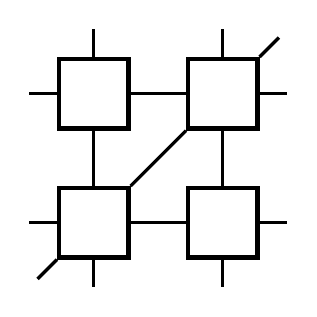
\begin{tikzpicture}
        \matrix [
            row sep=2em,
            column sep=2em,
            every node/.append style={draw, ultra thick, inner sep=0, minimum size=2.5em},
            ampersand replacement=\&,
        ] {%
          \node (core01) {}; \& \node (core11) {}; \\
          \node (core00) {}; \& \node (core10) {}; \\
        };

        % Connect the cores
        \foreach \i in {0, 1}{%
          \draw [very thick] (core0\i) -- (core1\i);
          \draw [very thick] (core\i0) -- (core\i1);

          \draw [very thick] (core0\i.west) -- ++(-1em, 0);
          \draw [very thick] (core1\i.east) -- ++(+1em, 0);
          \draw [very thick] (core\i0.south) -- ++(0, -1em);
          \draw [very thick] (core\i1.north) -- ++(0, +1em);
        };
        \draw [very thick] (core00.south west) -- ++(-.7em, -.7em);
        \draw [very thick] (core11.north east) -- ++(+.7em, +.7em);
        \draw [very thick] (core00) -- (core11);
      \end{tikzpicture}
    \end{column}
    \begin{column}{.7\textwidth}
      \begin{itemize}
        \item 18 cores per node
          \begin{itemize}
            \item \SI{64}{\kibi\byte} DTCM
            \item \SI{32}{\kibi\byte} ITCM
          \end{itemize}
        \item 1 router per node
          \begin{itemize}
            \item \textbf{1024 entry prioritized TCAM}
            \item \textit{Default routing}
          \end{itemize}
        \item Full machine
          \begin{itemize}
            \item \num{57600} nodes
            \item 1M cores
          \end{itemize}
      \end{itemize}
    \end{column}
  \end{columns}
\end{frame}

\begin{frame}{SpiNNaker Router Behavior}
  \begin{table}[H]
    \centering
    \begin{tabular}{c l}
      \toprule
      Key-Mask & Route \\
      \midrule
      \texttt{0000} & \texttt{NE N}\\
      \texttt{X111} & \texttt{S}\\
      \texttt{1XXX} & \texttt{3 4}\\
      \bottomrule
    \end{tabular}
  \end{table}

  \emph{Default-routed} packets travel in a straight line
  \vskip\baselineskip

  \textbf{What if tables are too big?}
\end{frame}

\begin{frame}{Benchmarks}
  \begin{center}
    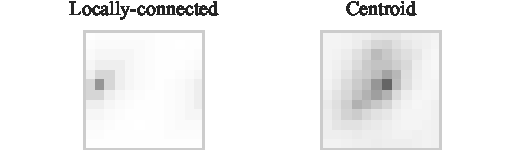
\includegraphics{../experiments/experiments}
  \end{center}

  Also --
  \begin{itemize}
    \item Broken links
  \end{itemize}
\end{frame}

\begin{frame}[plain]{}
  \begin{center}
    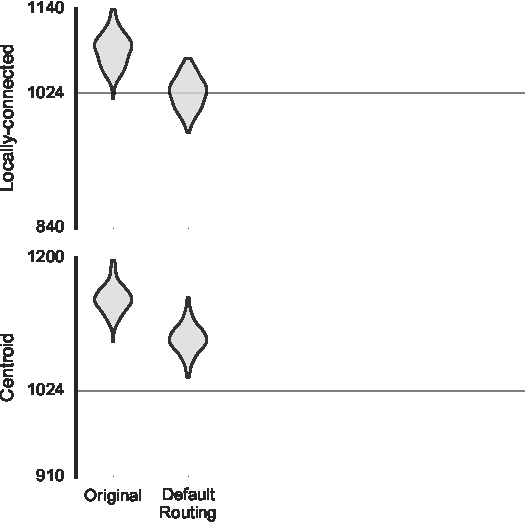
\includegraphics[page=1]{../experiments/presentation_plots}
  \end{center}
\end{frame}

\begin{frame}{Minimization with Espresso}  % Explanation
  \begin{columns}[T]
    \begin{column}{.5\textwidth}
      \begin{itemize}
        \item Break into subtables with the same route
        \item Minimize each subtable exactly
      \end{itemize}\vskip\baselineskip

      \textbf{Exact?}

      \texttt{0000} and \texttt{0001} $\rightarrow$ \texttt{000X}

      {\color{red} \texttt{0001} and \texttt{0010} $\rightarrow$ \cancel{\texttt{00XX}}}
    \end{column}
    \begin{column}{.5\textwidth}
      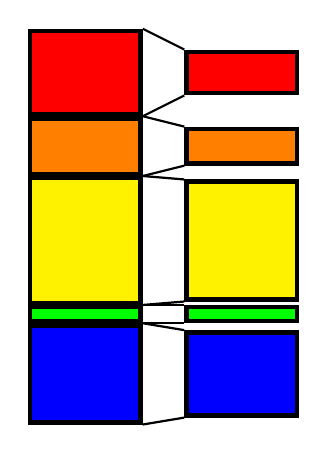
\begin{tikzpicture}[start chain=1 going below, node distance=0]
        % Diagram mostly of the form
        % A --> minimise exact --> a
        \foreach \X/\s/\t/\c in {
          A/3.0em/1.5em/red,
          B/2.0em/1.25em/orange,
          C/4.5em/4.25em/yellow,
          D/0.5em/0.50em/green,
          E/3.5em/3.00em/blue%
        }{
          \node (big\X) [subtable, minimum height=\s, fill=\c, on chain=1] {};
          \node (small\X) [subtable, minimum height=\t, fill=\c, right=1.5em of big\X] {};

          \draw [thick] (big\X.north east) -- (small\X.north west);
          \draw [thick] (big\X.south east) -- (small\X.south west);
        }
      \end{tikzpicture}
    \end{column}
  \end{columns}
\end{frame}

\begin{frame}[plain]{}
  \begin{center}
    \includegraphics[page=2]{../experiments/presentation_plots}
  \end{center}
\end{frame}

\begin{frame}{Minimization with Espresso}
  \begin{itemize}
    \item Good when coarse routing decisions can be made with few bits
      \begin{itemize}
        \item Source-based routing doesn't allow this
      \end{itemize}
    \item Ignores the prioritization of the TCAM
  \end{itemize}
\end{frame}

\begin{frame}{Order-exploiting minimization}  % With Espresso, explanation
  \begin{columns}[T]
    \begin{column}{.5\textwidth}
      \begin{itemize}
        \item Break into subtables with the same route
        \item \textbf{Sort in order of subtable size}
        \item Minimize each subtable \textbf{to avoid collisions with lower subtables}
      \end{itemize}\vskip.5\baselineskip

      \texttt{0001} and \texttt{0010} $\rightarrow$ \texttt{00XX} \emph{allowed} iff. no lower table contains \texttt{0000} or \texttt{0011}
    \end{column}
    \begin{column}{.5\textwidth}
      \only<1>{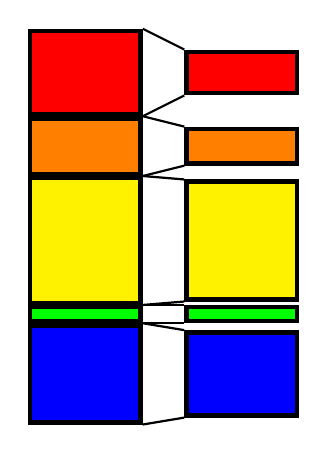
\begin{tikzpicture}[start chain=1 going below, node distance=0]
        % Diagram mostly of the form
        % A --> minimise exact --> a
        \foreach \X/\s/\t/\c in {
          A/3.0em/1.5em/red,
          B/2.0em/1.25em/orange,
          C/4.5em/4.25em/yellow,
          D/0.5em/0.50em/green,
          E/3.5em/3.00em/blue%
        }{
          \node (big\X) [subtable, minimum height=\s, fill=\c, on chain=1] {};
          \node (small\X) [subtable, minimum height=\t, fill=\c, right=1.5em of big\X] {};

          \draw [thick] (big\X.north east) -- (small\X.north west);
          \draw [thick] (big\X.south east) -- (small\X.south west);
        }
      \end{tikzpicture}}
      \only<2>{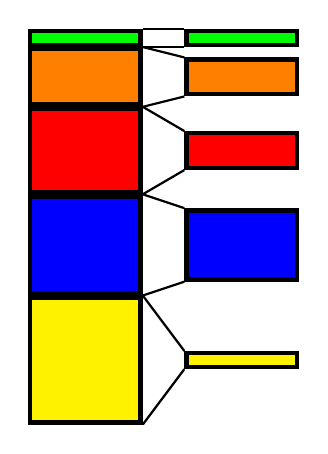
\begin{tikzpicture}[start chain=1 going below, node distance=0]
        % Same as before, but reordered according to original size
        \foreach \X/\s/\t/\c in {
          D/0.5em/0.50em/green,
          B/2.0em/1.25em/orange,
          A/3.0em/1.25em/red,
          E/3.5em/2.50em/blue,
          C/4.5em/0.50em/yellow%
        }{
          \node (big\X) [subtable, minimum height=\s, fill=\c, on chain=1] {};
          \node (small\X) [subtable, minimum height=\t, fill=\c, right=1.5em of big\X] {};

          \draw [thick] (big\X.north east) -- (small\X.north west);
          \draw [thick] (big\X.south east) -- (small\X.south west);
        }
      \end{tikzpicture}}
    \end{column}
  \end{columns}
\end{frame}

\begin{frame}[plain]{}
  \begin{center}
    \includegraphics[page=3]{../experiments/presentation_plots}
  \end{center}
\end{frame}

\begin{frame}{On-chip routing table minimization}  % Why?
  % Timing results from Espresso, assume naive scaling
  Espresso -- \SI{6.23}{\second} per table
  \pause $\times$ \num{57600} nodes\ldots
  \pause \emph{4 days}

  \begin{itemize}
    \item Problem is trivially parallel -- use SpiNNaker
    \item \textbf{BUT} Espresso \emph{is} big
    \item \textbf{AND} needs a lot of memory
  \end{itemize}

  Other people have looked at this:

  \begin{itemize}
    \item \fullcite{Lysecky2003}
    \item \fullcite{Ahmad2007} -- \textbf{m-Trie}
  \end{itemize}
\end{frame}

\begin{frame}[plain]{}
  \begin{center}
    \includegraphics[page=4]{../experiments/presentation_plots}
  \end{center}
\end{frame}

\begin{frame}{On-chip routing table minimization}
  Same problems as before --
  \begin{itemize}
    \item Good when coarse routing decisions can be made with few bits
    \item Ignores the prioritization of the TCAM
  \end{itemize}
  \vskip.5\baselineskip

  \textbf{Challenge}
  \begin{itemize}
    \item Simple minimizer (fit in ITCM)
    \item Small data structures (fit in DTCM)
    \item Exploit the ordering of the TCAM (minimize well)
  \end{itemize}
\end{frame}

\begin{frame}{Ordered-Covering}
  \centering
  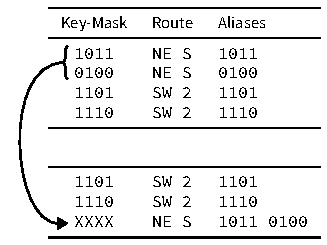
\includegraphics{aliases_example}

  \begin{itemize}
    \item Sort entries in ascending number of \texttt{X}s
    \item Annotate entries with keys they are expected to match
    \item Greedily merge entries with equivalent routes
      \begin{itemize}
        \item Subject to two rules\ldots
      \end{itemize}
  \end{itemize}
\end{frame}

\begin{frame}{\emph{Up-check} rule}
  No entry in the \emph{merge} may become \emph{covered} by another entry.

  \begin{center}
    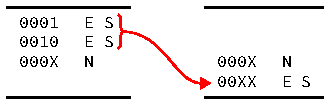
\includegraphics{../figures/rule2a_example}
  \end{center}

  e.g., \texttt{0011} becomes covered by \texttt{00XX}.
\end{frame}

\begin{frame}{\emph{Down-check} rule}
  No \emph{aliased entry} below the merge may become \emph{covered}.

  \begin{center}
    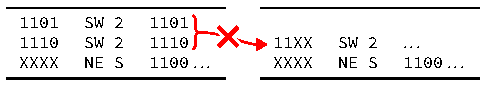
\includegraphics{../figures/rule2b_example}
  \end{center}

  e.g., \texttt{1100} becomes covered by \texttt{11XX}.
\end{frame}

\begin{frame}{Algorithm}
  \begin{itemize}
    \item While table is larger than desired
      \begin{itemize}
        \item Get the largest valid merge
        \item If the merge is empty, break
        \item Otherwise apply the merge
      \end{itemize}
  \end{itemize}

  Most potential merges will break the \emph{up-} or \emph{down-check} rules, so\ldots
\end{frame}

\begin{frame}{Resolving the \emph{up-check}}
  Remove from the merge any entry which would become \emph{covered} through being merged.

  \begin{center}
    \includegraphics<1>{../figures/upcheck_resolve_example_1}
    \includegraphics<2>{../figures/upcheck_resolve_example_2}
  \end{center}
\end{frame}

\begin{frame}{Resolving the \emph{down-check}}
  \begin{center}
    \only<1-2>{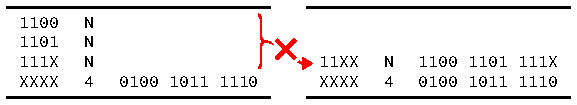
\includegraphics{../figures/downcheck_resolve_example_1}}
    \only<3>{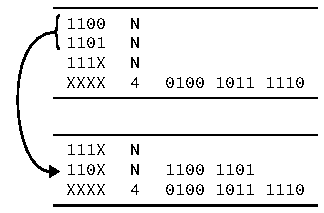
\includegraphics{../figures/downcheck_resolve_example_2}}
  \end{center}

  \only<1>{
  Convert an \texttt{X} to either \texttt{0} or \texttt{1}\ldots
  \vskip.5\baselineskip

  \texttt{0XXX} covers \texttt{0101} -- try to turn \texttt{0XXX} into:\\
    \hskip1em \texttt{0XX\underline{0}},
    \texttt{0X\underline{1}X} or
    \texttt{0\underline{0}XX}
  }
  \only<2-3>{\vskip-2.75\baselineskip
    \begin{align*}
      \{\texttt{0000},~\cancel{\texttt{0011}},~\cancel{\texttt{011X}}\} &~\rightarrow~ \texttt{000\underline{0}} \\
      \{\cancel{\texttt{0000}},~\texttt{0011},~\texttt{011X}\}          &~\rightarrow~ \texttt{0X\underline{1}X} \\
      \{\texttt{0000},~\texttt{0011},~\cancel{\texttt{011X}}\}          &~\rightarrow~ \texttt{0\underline{0}XX} \\
    \end{align*}
  }
\end{frame}

\begin{frame}[plain]{}
  \begin{center}
    \includegraphics[page=5]{../experiments/presentation_plots}
  \end{center}
\end{frame}

\begin{frame}{On-chip memory usage}
  Peak heap usage --
  \begin{center}
    \begin{tabular}{l S S}
      \toprule
      \textbf{Benchmark} & {\textbf{Total} / \si{\kibi\byte}} & {Table / \si{\kibi\byte}} \\
      \midrule
      Locally-connected & 18.4 & 13.3 \\
      Centroid          & 18.8 & 14.0 \\
      \bottomrule
    \end{tabular}
  \end{center}
  \vskip\baselineskip

  If reclaiming memory -- every merge of $\ge10$ entries decreases memory usage
\end{frame}

\begin{frame}{Timing}
  Ordered-Covering on SpiNNaker --
  \begin{center}
    \begin{tabular}{l S S S}
      \toprule
      & & \multicolumn{2}{c}{\textbf{Exec. time} / \si{\second}} \\
      \textbf{Model} & {\textbf{Load time} / \si{\second}} & {\textbf{Sufficient}} & {\textbf{Fully}} \\
      \midrule
      Locally-connected & 3.8 & 13.9 & 25.6 \\
      Centroid & 3.6 & & 25.6 \\
      \bottomrule
    \end{tabular}
  \end{center}

  \begin{itemize}
    \item Locally-connected benchmark -- 64.5$\times$ faster on SpiNNaker
    \item Centroid -- 2.8$\times$ faster
  \end{itemize}

  As networks scale\ldots
\end{frame}

\begin{darkframes}
  \begin{frame}{}
    \vfill
    \begin{center}
      {\huge Thank You}\\\vskip\baselineskip
      {\Large Any questions?}
    \end{center}
    \vfill
  \end{frame}

  \begin{frame}{Selected references}
    \begin{itemize}
      \item \fullcite{Furber2014}
      \item \fullcite{Navaridas2015}
      \item \fullcite{Liu2002}
    \end{itemize}
  \end{frame}
\end{darkframes}

\begin{frame}[plain]{}
  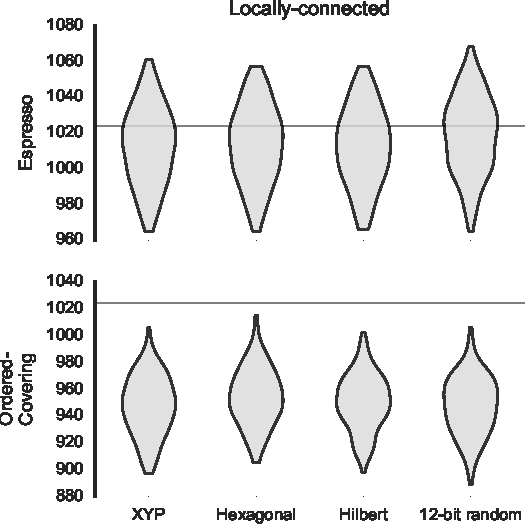
\includegraphics{keyspaces}
\end{frame}

\begin{frame}[c]{Using SpiNNaker}
  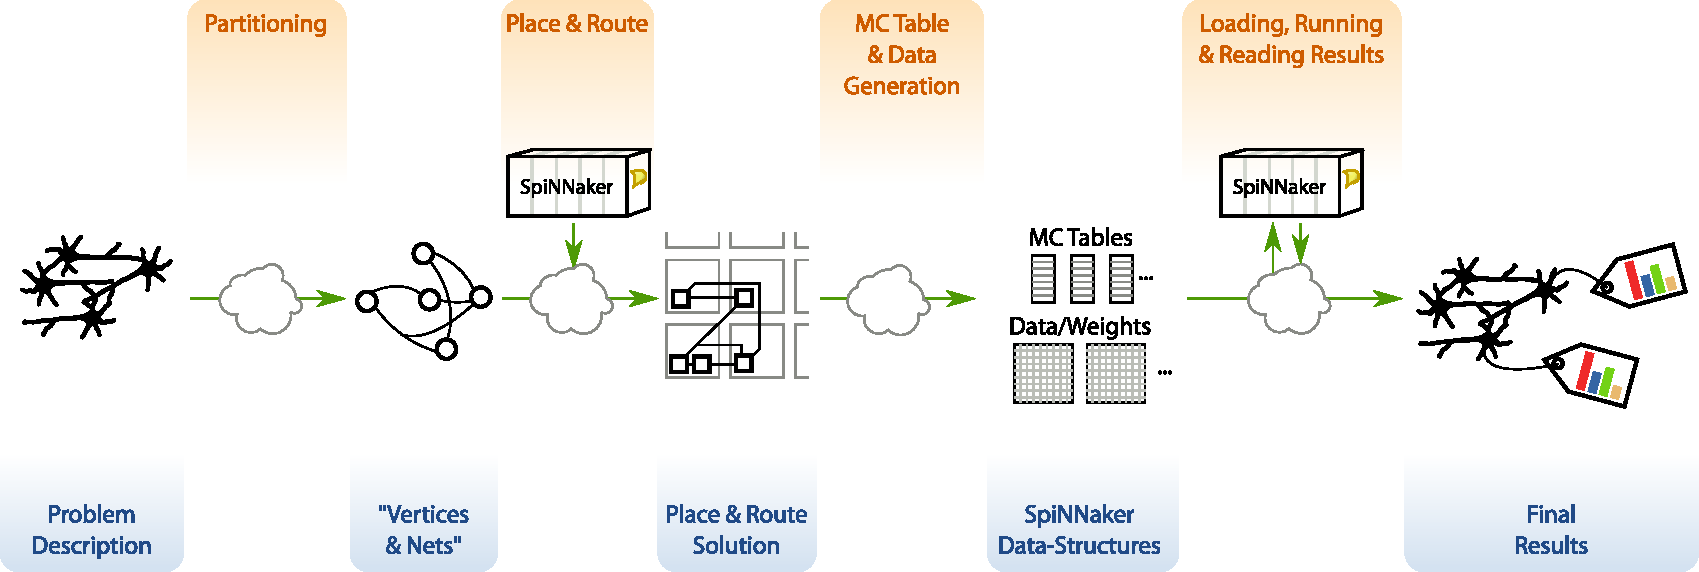
\includegraphics[width=\textwidth]{typical_application}
\end{frame}

\begin{frame}[c]{Using SpiNNaker (2)}
  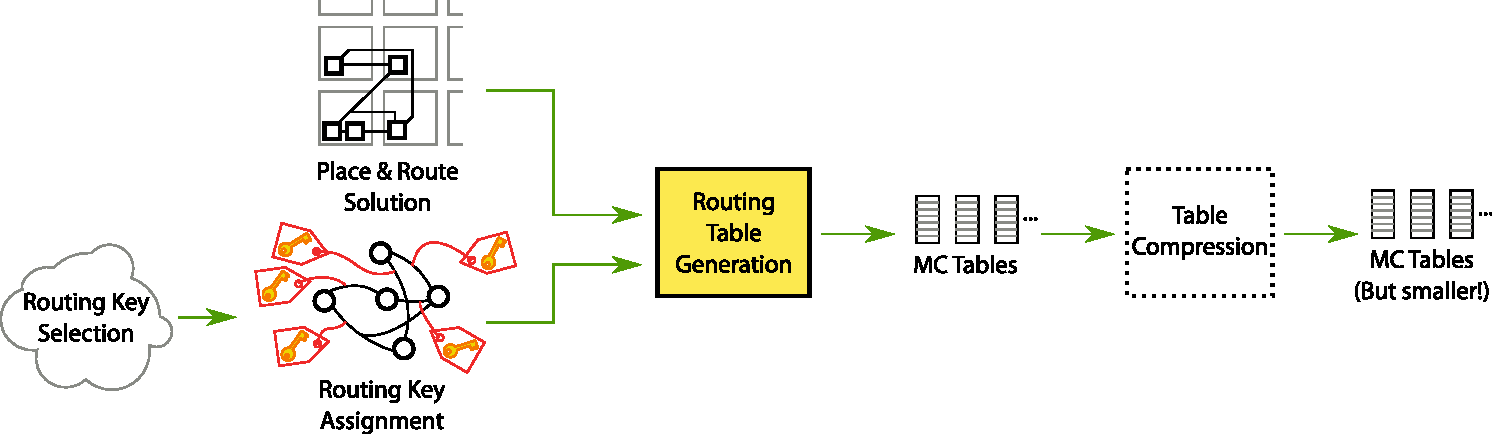
\includegraphics[width=\textwidth]{table_and_data_gen}
\end{frame}

\begin{darkframes}
  \begin{frame}[c]{(Half)-SpiNNaker}
    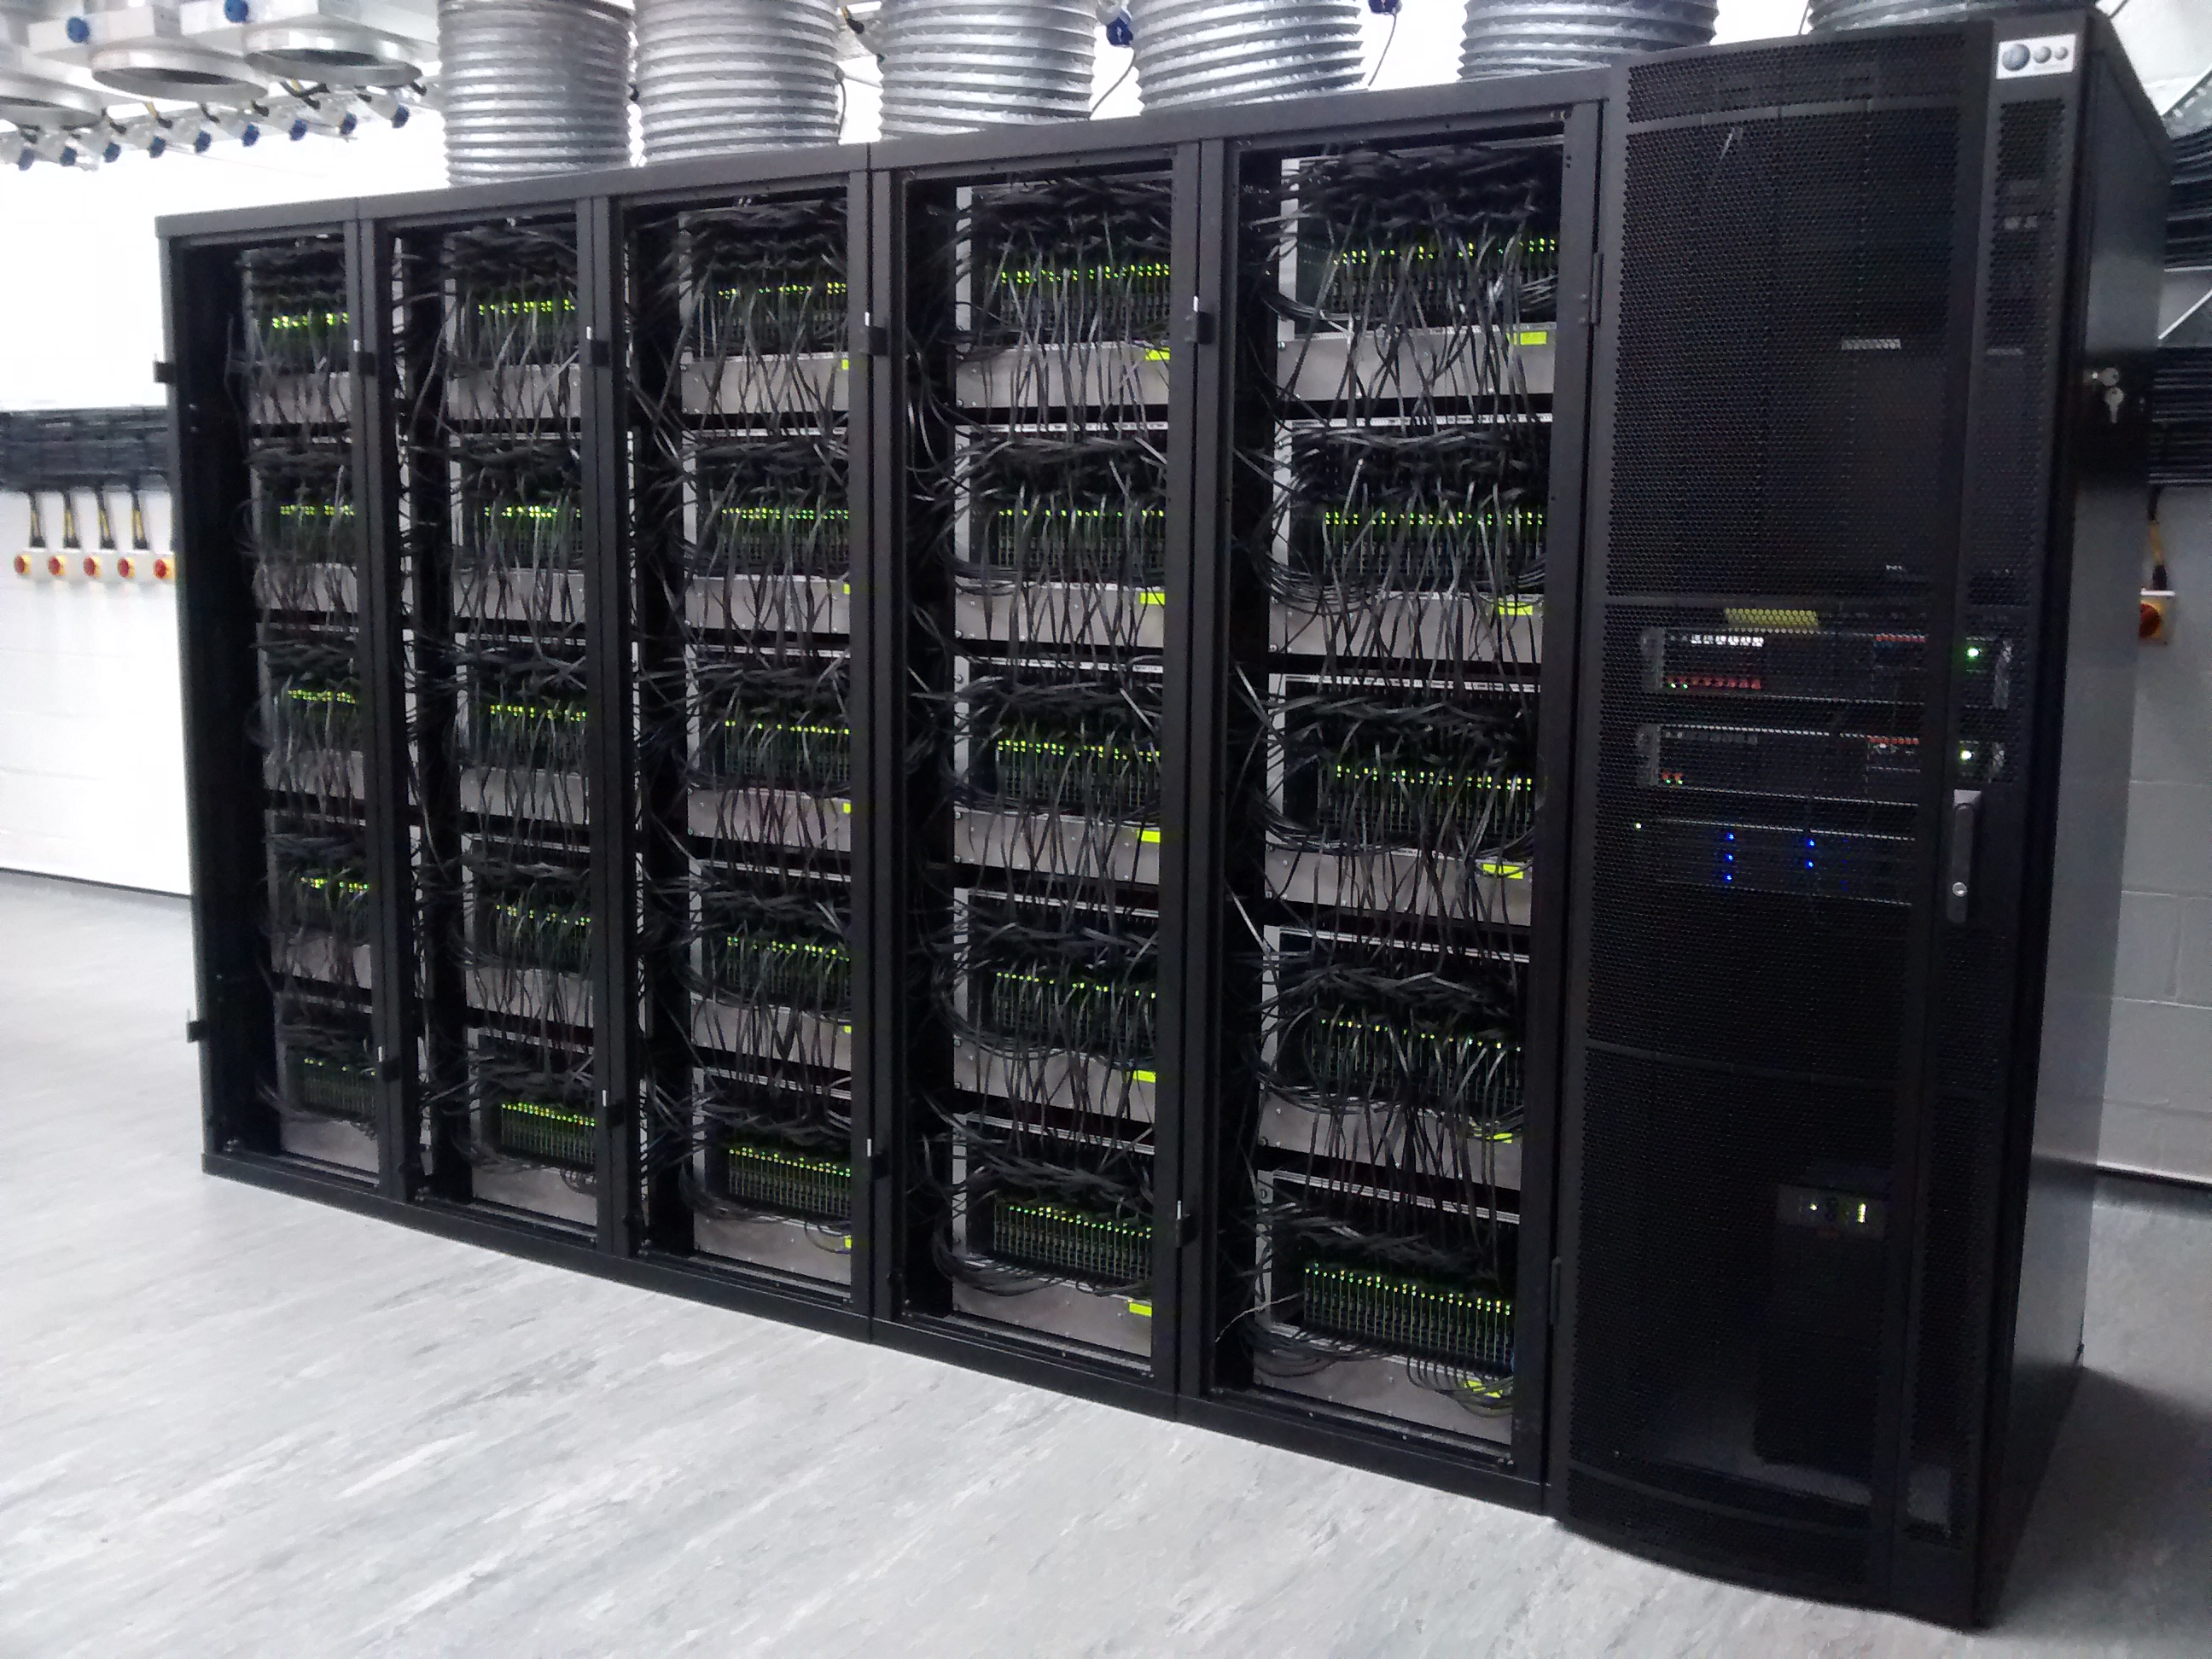
\includegraphics[width=\textwidth]{SpiNNaker}
  \end{frame}
\end{darkframes}
\end{document}
